\chapter{qmake Manual}
The qmake tool helps simplify the build process for development projects across different platforms.%
It automates the generation of Makefiles so that only a few lines of information are needed to create each Makefile.%
You can use qmake for any software project, whether it is written with Qt or not.%
\par
qmake generates a Makefile based on the information in a project file. Project files are created by the developer, and are usually simple, but more sophisticated project files can be created for complex projects.
\par
qmake contains additional features to support development with Qt, automatically including build rules for moc and uic.%
qmake can also generate projects for Microsoft Visual studio without requiring the developer to change the project file.

\section{Overview}
The qmake tool provides you with a project-oriented system for managing the build process for applications, libraries, and other components. This approach gives you control over the source files used, and allows each of the steps in the process to be described concisely, typically within a single file. qmake expands the information in each project file to a Makefile that executes the necessary commands for compiling and linking.

\subsection{Describing a project}
Projects are described by the contents of project (.pro) files. qmake uses the information within the files to generate Makefiles that contain all the commands that are needed to build each project. Project files typically contain a list of source and header files, general configuration information,
and any application-specific details, such as a list of extra libraries to link against, or a list of extra include paths to use.
\par
Project files can contain a number of different elements, including comments, variable declarations, built-in functions, and some simple control structures. In most simple projects, it is only necessary to declare the source and header files that are used to build the project with some basic
configuration options. For more information about how to create a simple project file, see Getting Started.
\par
You can create more sophisticated project files for complex projects. For an overview of project files, see Creating Project Files. For detailed information about the variables and functions that you can use in project files, see Reference.
\par
You can use application or library project templates to specify specialized configuration options to fine tune the build process. For more information, see Building Common Project Types.
\par
You can use the Qt Creator new project wizard to create the project file. You choose the project template, and Qt Creator creates a project file with default values that enable you to build and run the project. You can modify the project file to suit your purposes.
\par
You can also use qmake to generate project files. For a full description of qmake command line options, see Running qmake.
\par
The basic configuration features of qmake can handle most cross-platform projects. However, it might be useful, or even necessary, to use some platform-specific variables. For more information, see Platform Notes.

\subsection{创建一个项目文件}
qmake使用储存在项目(.pro)文件中的信息来决定Makefile文件中该生成什么。\par
一个基本的项目文件包含关于应用程序的信息,比如,编译应用程序需要哪些文件,并且使用哪些配置设置。\par
这里是一个简单的示例项目文件:
\begin{flushleft}
  {\color{seagreen}{
      SOURCES = hello.cpp \\
      HEADERS = hello.h \\
      CONFIG += qt warn\_on release
    }}
\end{flushleft}
我们将会提供一行一行的简要解释,具体细节将会在手册的后面的部分解释。\\
{\color{seagreen}{
    SOURCES = hello.cpp
  }}\\
这一行指定了实现应用程序的源程序文件。在这个例子中,恰好只有一个文件,hello.cpp。大部分应用程序需要多个文件,这种情况下可以把文件列在一行中,以空格分隔,就像这样:\\
{\color{seagreen}{
    SOURCES = hello.cpp main.cpp
  }}\\
另一种方式,每一个文件可以被列在一个分开的行里面,通过反斜线另起一行,就像这样:\\
{\color{seagreen}{
    SOURCES = hello.cpp $\backslash$ \\
    \hspace*{2.5cm}main.cpp
  }}\\
一个更冗长的方法是单独地列出每一个文件,就像这样:\\
{\color{seagreen}{
    SOURCES += hello.cpp\\
    SOURCES += main.cpp
  }}\\
这种方法中使用“+=”比“=”更安全,因为它只是向已有的列表中添加新的文件,而不是替换整个列表。\par
HEADERS这一行中通常用来指定为这个应用程序创建的头文件,举例来说:\\
{\color{seagreen}{
    HEADERS += hello.h
  }}\\
列出源文件的任何一个方法对头文件也都适用。\\
CONFIG这一行是用来告诉qmake关于应用程序的配置信息。\\
{\color{seagreen}{
    CONFIG += qt warn\_on release
  }}\\
在这里使用“+=”,是因为我们添加我们的配置选项到任何一个已经存在中。这样做比使用“=”那样替换已经指定的所有选项是更安全的。\par
CONFIG一行中的qt部分告诉qmake这个应用程序是使用Qt来连编的。这也就是说qmake在连接和为编译添加所需的包含路径的时候会考虑到Qt库的。\par
CONFIG一行中的warn\_on部分告诉qmake要把编译器设置为输出警告信息的。\par
CONFIG一行中的release部分告诉qmake应用程序必须被连编为一个发布的应用程序。在开发过程中,程序员也可以使用debug来替换release,稍后会讨论这里的。\par
项目文件就是纯文本(比如,可以使用像记事本、vim和xemacs这些编辑器)并且必须存为“.pro”扩展名。应用程序的执行文件的名称必须和项目文件的名称一样,但是扩展名是跟着平台而改变的。举例来说,一个叫做“hello.pro”的项目文件将会在Windows下生成“hello.exe”,而在Unix下生成“hello”。

\subsection{生成Makefile}
当你已经创建好你的项目文件,生成Makefile就很容易了,你所要做的就是先到你所生成的项目文件那里然后输入:\\
Makefile可以像这样由“.pro”文件生成:\\
{\color{seagreen}{
    qmake -o Makefile hello.pro
  }}\\
对于Visual Studio的用户,qmake也可以生成“.dsp”文件,例如:\\
{\color{seagreen}{
    qmake -t vcapp -o hello.dsp hello.pro

  }}

\section{开始}
这篇教程会讲述qmake的基础,这本手册的其他主题包含了有关使用qmake的更多信息。
\subsection{简单的开始}
假设你已经完成了你的应用的基本实现,并且你已经创建了如下文件:
\begin{itemize}
\item{hello.cpp}
\item{hello.h}
\item{main.cpp }
\end{itemize}
首先,在源代码所在的目录用纯文本编辑器创建一个叫hello.pro的文本文件,你要做的第一件事
是在该文件中添加几行来告诉qmake这些源文件和头文件是你的项目中的一部分。
我们首先要添加源文件到项目中,为达成这个目的你需要使用”SOURCES“变量,将hello.cpp
加入项目可以这样做。\\
{\color{seagreen}{
    SORUCES += hello.cpp
  }}\\
如果你更喜欢make风格的语法,即一次列出所有文件,你可以使用换行符,就像这样: \\
{\color{seagreen}{
    SOURCES += hello.cpp $\backslash$ \\
    \hspace*{2.5cm}main.cpp
  }}\\
既然源文件已经被列入项目文件中了,那么头文件也必须被添加。他们的添加方式与源文件完全
相同,除了变量名叫“HEADERS” \\
当你做完这些事后,你的项目文件应当是这样的:\\
{\color{seagreen}{
    HEADERS += hello.h\\
    SOURCES += hello.cpp\\
    SOURCES += main.cpp
  }}\\
目标名称会自动设置,它与项目文件名相同,只是会添加适合与平台的后缀。例如,如果项目文件
叫做hello.pro,在Windows上目标将会叫做hello.exe,而在Unix上叫hello。如果你想使用
一个不同的名字的话可以在项目文件中设置:\\
{\color{seagreen}{
    TARGET = helloworld
  }}\\
你可以使用qmake来为你的应用生产makefile,在命令行界面,进入项目目录,输入下列命令:\\
{\color{seagreen}{
    qmake -o Makefile hello.pro
  }}
然后根据你使用的编译器输入’make‘或’nmake‘。

\subsection{使应用支持调试}























\subsection{Starting Off Simple}
Let's assume that you have just finished a basic implementation of your application, and you have created the following files:
\begin{itemize}
\item{hello.cpp}
\item{hello.h}
\item{main.cpp}
\end{itemize}
You will find these files in the examples/qmake/tutorial directory of the Qt distribution. The only other thing you know about the setup of the application is that it's written in Qt. First, using your favorite plain text editor, create a file called hello.pro in examples/qmake/tutorial. The first
thing you need to do is add the lines that tell qmake about the source and header files that are part of your development project.
\par
We'll add the source files to the project file first. To do this you need to use the SOURCES variable. Just start a new line with SOURCES += and put hello.cpp after it. You should have something like this:
\begin{center}
  {\color{seagreen}{SOURCES += hello.cpp}}
\end{center}
We repeat this for each source file in the project, until we end up with the following:
\begin{center}
  {\color{seagreen}{SOURCES += hello.cpp\\
      SOURCES += main.cpp}}
\end{center}
If you prefer to use a Make-like syntax, with all the files listed in one go you can use the newline escaping like this:
\begin{center}
  {\color{seagreen}{SOURCES = hello.cpp $\backslash$ \\
      \hspace*{2.5cm}main.cpp}}
\end{center}
Now that the source files are listed in the project file, the header files must be added. These are added in exactly the same way as source files, except that the variable name we use is HEADERS.\\
Once you have done this, your project file should look something like this:
\begin{center}
{\color{seagreen}{SOURCES = hello.cpp $\backslash$ \\
    \hspace*{2.5cm}main.cpp\\
    HEADERS += hello.h
  }}
\end{center}
The target name is set automatically. It is the same as the project filename, but with the suffix appropriate for the platform. For example, if the project file is called hello.pro, the target will be hello.exe on Windows and hello on Unix. If you want to use a different name you can set it in the
project file:
\begin{center}
  {\color{seagreen}{TARGET = helloworld}}
\end{center}
The finished project file should look like this:
\begin{center}
  {\color{seagreen}{HEADERS += hello.h\\
      SOURCES += hello.cpp\\
      SOURCES += main.cpp}}
\end{center}
You can now use qmake to generate a Makefile for your application. On the command line, in your project directory, type the following:
\begin{center}
  {\color{seagreen}{qmake -o Makefile hello.pro}}
\end{center}
Then type make or nmake depending on the compiler you use.
\par
For Visual Studio users, qmake can also generate Visual Studio project files. For example:
\begin{center}
  {\color{seagreen}{qmake -tp vc hello.pro}}
\end{center}

\section{Making an Application Debuggable}
The release version of an application does not contain any debugging symbols or other debugging information. During development, it is useful to produce a debugging version of the application that has the relevant information. This is easily achieved by adding debug to the CONFIG variable in the
project file.
\par
For example:
\begin{center}
  \color{seagreen}
  CONFIG += debug\\
  HEADERS += hello.h\\
  SOURCES += hello.cpp\\
  SOURCES += main.cpp
\end{center}
Use qmake as before to generate a Makefile. You will now obtain useful information about your application when running it in a debugging environment.

\section{Adding Platform-Specific Source Files}
After a few hours of coding, you might have made a start on the platform-specific part of your application, and decided to keep the platform-dependent code separate. So you now have two new files to include into your project file: hellowin.cpp and hellounix.cpp. We cannot just add these to the
SOURCES variable since that would place both files in the Makefile. So, what we need to do here is to use a scope which will be processed depending on which platform we are building for.
\par
A simple scope that adds the platform-dependent file for Windows looks like this:
\begin{center}
  {\color{seagreen}{
      \begin{lstlisting}
        win32 {
          SOURCES += hellowin.cpp
        }
      \end{lstlisting}}}
\end{center}
When building for Windows, qmake adds hellowin.cpp to the list of source files. When building for any other platform, qmake simply ignores it. Now all that is left to be done is to create a scope for the Unix-specific file.
\par
When you have done that, your project file should look something like this:
\begin{center}
  {\color{seagreen}
    {
      \begin{lstlisting}
        CONFIG += debug
        HEADERS += hello.h
        SOURCES += hello.cpp
        SOURCES += main.cpp
        win32 {
          SOURCES += hellowin.cpp
        }
        unix {
          SOURCES += hellounix.cpp
        }
      \end{lstlisting}
    }}
\end{center}
Use qmake as before to generate a Makefile.\\
The ! symbol is used to negate the test. That is, exists( main.cpp ) is true if the file exists, and !exists( main.cpp ) is true if the file does not exist.
\begin{center}
  {\color{seagreen}{
      \begin{lstlisting}
        CONFIG += debug
        HEADERS += hello.h
        SOURCES += hello.cpp
        SOURCES += main.cpp
        win32 {
          SOURCES += hellowin.cpp
        }
        unix {
          SOURCES += hellounix.cpp
        }
        !exists( main.cpp ) {
          error( "No main.cpp file found" )
        }
      \end{lstlisting}
    }}
\end{center}
Use qmake as before to generate a makefile. If you rename main.cpp temporarily, you will see the message and qmake will stop processing.

\section{Checking for More than One Condition}
Suppose you use Windows and you want to be able to see statement output with qDebug() when you run your application on the command line. To see the output, you must build your application with the appropriate console setting. We can easily put console on the CONFIG line to include this setting in
the Makefile on Windows. However, let's say that we only want to add the CONFIG line when we are running on Windows and when debug is already on the CONFIG line. This requires using two nested scopes. First create one scope, then create the other inside it. Put the settings to be processed inside
the second scope, like this:
\begin{center}
  {\color{seagreen}{
      \begin{lstlisting}
        win32 {
          debug {
            CONFIG += console
          }
        }
      \end{lstlisting}
    }}
\end{center}
Nested scopes can be joined together using colons, so the final project file looks like this:
\begin{center}
  {\color{seagreen}{
      \begin{lstlisting}
        CONFIG += debug
        HEADERS += hello.h
        SOURCES += hello.cpp
        SOURCES += main.cpp
        win32 {
          SOURCES += hellowin.cpp
        }
        unix {
          SOURCES += hellounix.cpp
        }
        !exists( main.cpp ) {
          error( "No main.cpp file found" )
        }
        win32:debug {
          CONFIG += console
        }
      \end{lstlisting}
    }}
\end{center}
That's it! You have now completed the tutorial for qmake, and are ready to write project files for your development projects.

\section{创建项目文件}
项目文件通常包含创建应用程序,库和插件所需要的一切信息。%
Generally, you use a series of declarations to specify the resources in the project,
but support for the simple programming constructs enables you to describe different build processes for
different platforms and evvironments.

\subsection{项目文件的elements}
The project file format used by qmake can be to support both simple and fairly complex build systems(简单复杂的通吃)。%
对于简单的项目文件而言,使用直接的变量声明的方式,定义标准的变量来表明哪些头文件和源文件会被用到。%
复杂的项目文件或许用到控制流结构来fine-tune the build process.%
\\\newline
下面的sections描述项目文件中被用到的不同元素类型。%

\subsubsection{变量}
在项目文件中,变量被用来保存字符串的一个列表。%
在最简单的项目中,这些变量告诉qmake哪些配置选项会被使用,%
或者在创建过程中要被用到的文件名或者路径。
\\\newline
qmake在每一个项目文件中寻找确定的变量,%
并用它们的内容来决定在哪些东西应该被用来写到Makefile文件中。%
例如,{\color{seagreen}{HEADERS和SOURCES}}变量被用来告诉qmake在相同的目录下哪些头文件和源文件会被当前的项目文件用到。%
\newline

下面的snippets展示了如何给变量进行赋值:
\begin{figure}[htbp]
  \centering
  
\includegraphics[width=\textwidth]{qmake/images/headers}
\end{figure}

多行变量内容采用下面的方式进行书写:(反斜线连接)
\begin{figure}[htbp]
  \centering
  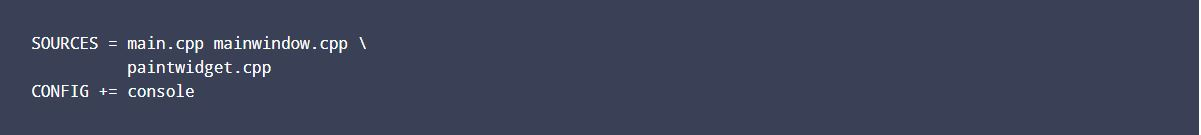
\includegraphics[width=\textwidth]{qmake/images/sources}
\end{figure}

下表是经常被用到的变量以及对它们变量内容的讨论。
\begin{table}[htbp]
  \centering
  \begin{tabular}{|l|l|}\hline
    变量 & 内容 \\\hline
    {\color{seagreen}{CONFIG}} & 一般项目配置选项 \\\hline
    {\color{seagreen}{DESTID}} & 生成的可执行文件的存放目录 \\\hline
    {\color{seagreen}{FORMS}}  & UI文件的列表 \\\hline
    {\color{seagreen}{HEADERS}} & 头文件列表 \\\hline
    {\color{seagreen}{QT}}     & 模块内容列表 \\\hline
    {\color{seagreen}{RESOURCES}} & 资源文件列表 \\\hline
    {\color{seagreen}{SOURCES}} & 源文件列表 \\\hline
    {\color{seagreen}{TEMPLATE}} & 项目文件的类型(可能是可执行程序,库或者插件) \\\hline
  \end{tabular}
\end{table}

其中\$\$两个美元符号被用来作为内建函数,变量的引用的展开。

\subsubsection{空格}
通常空格是被忽略的,如果想显式的使用空格,必须用双引号进行括起来。
如:
\begin{figure}[htbp]
  \centering
  
\includegraphics[width=\textwidth]{qmake/images/whitespace1}
\end{figure}

\begin{figure}[htbp]
  \centering
  
\includegraphics[width=\textwidth]{qmake/images/whitespace2}
\end{figure}

\subsubsection{注释}
注释使用shape(\#)符号进行注释

\subsubsection{内建函数和控制流}
qmake提供了一组内建的函数来处理变量的内容,如最常用的include函数,%
其中include函数被用来包含其它的项目文件:
\begin{figure}[htbp]
  \centering
  
\includegraphics[width=\textwidth]{qmake/images/include}
\end{figure}

对于变量更加复杂的操作需要可能要用到循环,如find(), unique()和count().

\subsection{项目template}
变量{\color{seagreen}{TEMPLATE}}被用来指定该项目的生成类型,%
缺省的项目类型是app。%

下图是项目类型列表:
\begin{table}[htbp]
  \centering
  \begin{tabular}{|l|l|} \hline
    Template          & qmake Output \\\hline
    app(default)      & 生成application \\\hline
    lib               & 创建库 \\\hline
    aux               & Makefile to build nothing \\\hline
    subdirs           & subdirs指定包含的子目录,每个子目录必须有自己的项目文件 \\\hline
    vcapp             & 创建 Visual Studio的应用程序 \\\hline
    vclib             & 创建 Visual Studio的库  \\\hline
    vcsubdirs         & Visual Studio Solution file to build project in sub-directories \\\hline
  \end{tabular}
\end{table}


\subsection{一般配置}
变量{\color{seagreen}{CONFIG}}指定项目的options和特征。

项目可以被指定为release版本,也可以指定为debug版本,%
如果两个都指定将以最后一个为创建的依据,%
如果两个版本的方式都想指定,可以将值改为{\color{seagreen}{debug\_and\_release}}

\textbf{Note:} Each of the options specialized in the \textbf{CONFIG} variable can also be used as a scope condition.%
you can test for the presence of certain configuration options by using the built-in {\color{seagreen}CONFIG()} function.%
For example, the following lines show the function as the condition in a scope to test whether only the opengl option is in use:
\begin{figure}[htbp]
  \centering
  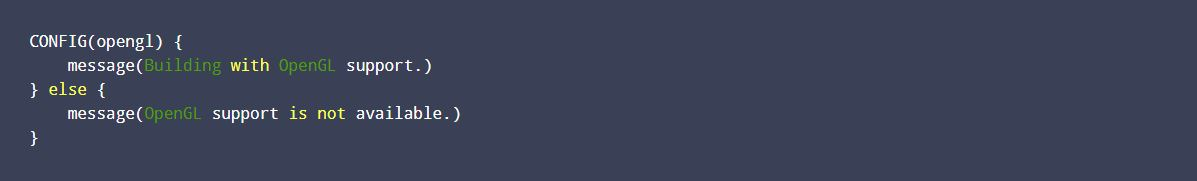
\includegraphics[width=\textwidth]{qmake/images/opengl}
\end{figure}

下面的options定义项目创建的类型:
\begin{table}[htbp]
  \centering
  \begin{tabular}{|l|l|} \hline
    \textbf{选项}   & \textbf{描述} \\\hline
    qt              & 该项目是一个Qt应用程序,且应该连接Qt库。 \\\hline
    x11             & 该项目是一个x11应用程序。\\\hline
  \end{tabular}
\end{table}

如果你的应用程序使用Qt库也想是debug版本,你可以采用以下的配置:


\subsection{声明Qt库}
我们可以使用变量{\color{seagreen}QT}来确定要使用哪些模块,如下面的例子:
\begin{figure}[htbp]
  \centering
  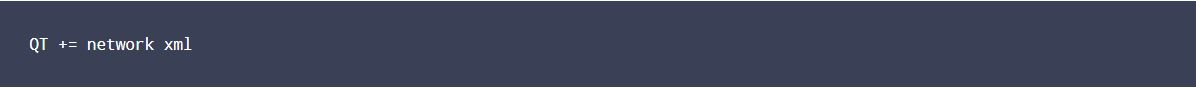
\includegraphics[width=\textwidth]{qmake/images/zhuijia}
\end{figure}

其中QT缺省值是包含core和gui这两个模块的。

使用下面的方式,将会忽略掉core和gui两个模块。
\begin{figure}[htbp]
  \centering
  
\includegraphics[width=\textwidth]{qmake/images/fuzhi}
\end{figure}

但是我们也可以显式的去掉缺省的模块,如下面的方式:
\begin{figure}[htbp]
  \centering
  
\includegraphics[width=\textwidth]{qmake/images/jianqu}
\end{figure}

\subsection{声明其它的库}
我们可以使用变量{\color{seagreen}LIBS}来添加其它的库,如:
\begin{figure}[htbp]
  \centering
  
\includegraphics[width=\textwidth]{qmake/images/libs}
\end{figure}

其它头文件的指定方式我们可以指定其搜索的目录,如:
\begin{figure}[htbp]
  \centering
  
\includegraphics[width=\textwidth]{qmake/images/headers_path}
\end{figure}





%%% Local Variables:
%%% mode: latex
%%% TeX-master: t
%%% End:
